\section{A brief history of DNA}

In the winter of 1868/9, Swiss physician and biologist, Johannes Friedrich Miescher isolated an unknown substance from the nuclei of cells \citep{dahm2008discovering}. This substance was unlike anything he had observed before; it was resistant to protease, lacked sulphur, and contained a large amount of phosphorous. He recognised that he had isolated a novel substance and as it was from the nucleus, he named it nuclein. In 1881, Albrecht Kossel determined that nuclein was composed of five bases: adenine (A), cytosine (C), guanine (G), thymine (T), and uracil (U). Later in 1889, Richard Altmann discovered that nuclein was acidic (due to the presence of phosphorous) and renamed nuclein to nucleic acid. The basic component of deoxyribonucleic acid (DNA) was deduced by Phoebus Levene in 1909, who discovered that DNA consisted of an acid, an organic base, and a sugar. Levene also showed that these components were linked together as phosphate-sugar-base to form units, which he termed nucleotides. This sugar-phosphate backbone forms the structural framework of nucleic acids and makes DNA highly stable. In 1928, Frederick Griffith demonstrated that heritable traits could be transferred between dead and live bacteria and that provided the first clue that a ``transforming factor" existed \citep{griffith1928significance}. It wasn't until 1944, when Oswald Avery, Colin MacLeod, and Maclyn McCarty demonstrated that deoxyribonucleo-depolymerase (an enzyme that degrades DNA) destroyed the ``transforming factor", that DNA was hypothesised as the genetic material that allowed the transformation \citep{avery1944studies}. This was later confirmed in 1952 by Alfred Hershey and Martha Chase, by demonstrating that when bacteriophages infected bacteria, only their DNA would enter into the cytoplasm of the bacteria, while their protein remained external to the cell \citep{hershey1952independent}.

While Levene proposed that DNA was made up of equal amounts of A, C, G, and T, it was later discovered by Erwin Chargaff that DNA had a one-to-one ratio of pyrimidine (C, T, and U) and purine (A and G) bases \citep{pmid14938364, pmid14945441}; this became known as Chargaff's rules. This observation by Chargaff and insights gained from Rosalind Franklin were necessary for the deduction of the three-dimensional (3D) structure of DNA by Francis Crick and James Watson in 1953 \citep{WATSON_1953}. The 3D structure of DNA demonstrated how adenines paired with thymines and cytosines paired with guanines (Figure ~\ref{fig:dna}); this became known as Watson-Crick base pairing and explained how genetic information could be copied due to the complementary nature of DNA.

\begin{figure}[!ht]
   \centering
   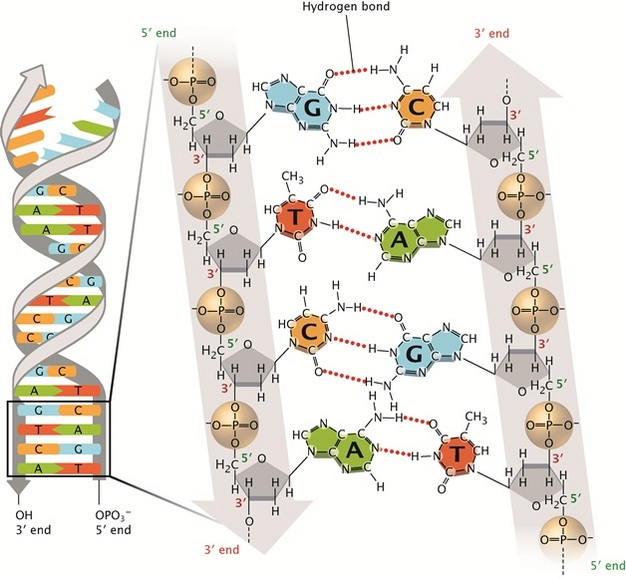
\includegraphics[width=\textwidth, natwidth=626, natheight=579, totalheight=0.40\textheight, keepaspectratio]{dna_scitable.jpg}
   \caption[DNA base pairing]{The structure of DNA is based on the repeated pattern of deoxyriboses and phosphate groups, forming the sugar-phosphate backbone, and the base pairing of the four bases, adenine (A), cytosine (C), guanine (G), and thymine (T). Two hydrogen bonds connect A's to T's and three hydrogen bonds connect C's to G's. Image used with permission from Nature Education 2013.}
   \label{fig:dna}
\end{figure}

\section{The Central Dogma of Molecular Biology}
\label{sec:central_dogma}

In 1958, Francis Crick wrote a seminal paper on protein synthesis, where he described the importance of proteins in living organisms and first proposed the central dogma of molecular biology \citep{crick1958protein}. Crick described how DNA or ribonucleic acid (RNA) could be used as templates for proteins and further described the possible directions of information flow between DNA, RNA, and protein. However, he noted that once information had been transferred from either DNA or RNA to protein, it was not possible for this information to flow back to nucleic acids (Figure ~\ref{fig:central_dogma}). In 1970, an enzyme now known as reverse transcriptase (RT) was discovered \citep{pmid4316301,pmid4316300}, which allowed RNA to be used as a template for producing DNA. In light of this and due to the misunderstanding of the central dogma, Crick restated the central dogma emphasising the information flow between the molecules \citep{CRICK1970}: ``The central dogma of molecular biology deals with the detailed residue-by-residue transfer of sequential information. It states that such information cannot be transferred from protein to either protein or nucleic acid."

\begin{figure}[!ht]
   \centering
   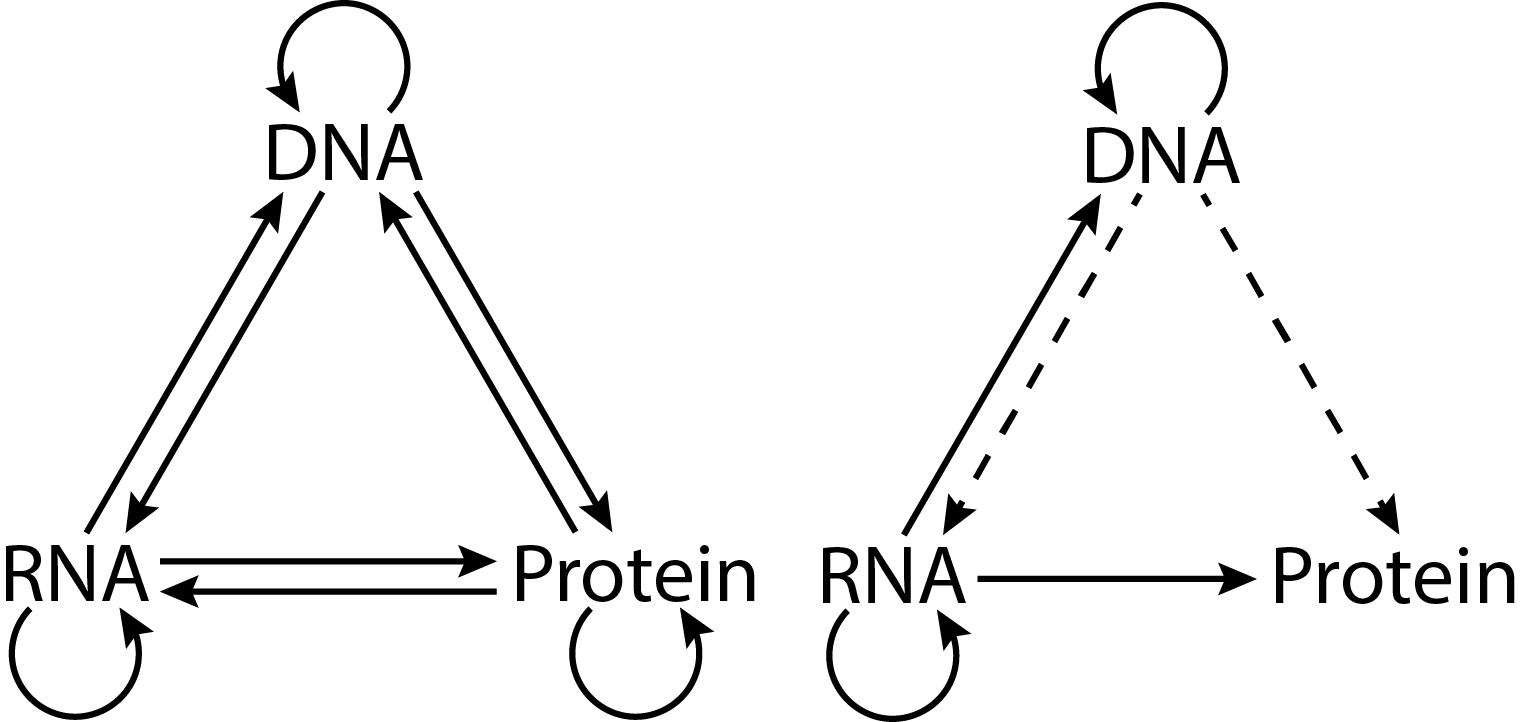
\includegraphics[width=\textwidth,natwidth=1520,natheight=722,totalheight=0.20\textheight,keepaspectratio]{central_dogma.png}
   \caption[The central dogma]{The central dogma of molecular biology depicting all possible information transfer pathways between DNA, RNA, and protein are shown on the left. Probable (solid arrows) and possible (dotted arrows) information transfer pathways, as originally proposed in 1958 by Francis Crick \citep{crick1958protein}, are shown on the right.}
   \label{fig:central_dogma}
\end{figure}

Prior to proposing the central dogma, Crick had predicted the existence of ``adaptors" that would transfer information from RNA to protein in 1955 \citep{cricktrna1955}. Crick proposed that there were twenty adaptors and special enzymes, one for each amino acid; the enzymes would join a particular amino acid to its own special adaptor. This theory was later confirmed by the discovery of transfer RNA (tRNA) in 1958 \citep{pmid13538965}. The discovery of messenger RNA (mRNA) in 1961 \citep{BRENNER1961} demonstrated how genetic information from DNA could be transferred to the ribosomes. In 1962, characteristics of how DNA encoded amino acid sequences of proteins was revealed with the development of a cell-free protein synthesising system \citep{pmid14471390}. Matthaei and colleagues demonstrated that an artificially created RNA, composed entirely of uracils, would produce a protein composed entirely of phenylalanine. The full code, known as the genetic code, was cracked three years later in 1965 \citep{pmid5330357} and defined how information was encoded in DNA to produce amino acids. Nirenberg and colleagues deduced that three nucleotides defined a codon, which are translated into one of the 20 standard amino acids.

\section{Transcription}

Transcription is the process by which a particular segment of DNA is processed into RNA by the enzyme RNA polymerase (RNA pol). There are three different types of RNA pols in eukaryotic cells: Pol I transcribes DNA that encode most of the ribosomal RNAs (rRNAs); Pol II transcribes DNA that encode mRNAs and other non-coding RNAs (ncRNAs); and Pol III transcribes DNA that encode small regulatory RNA molecules, such as tRNAs. The first step in transcription is initiation, whereby RNA pol binds upstream of the DNA to be transcribed, at a region known as the promoter (Figure ~\ref{fig:transcription}). The main role of the promoter is to bind and position the transcription initiation complex, which contains the RNA pol. Classically, promoters were classified mainly by their proximity to the transcription start site (TSS), which are the first nucleotides transcribed by RNA pol. In eukaryotes, the core promoter is often defined as the DNA region in the immediate vicinity of the TSS and contains interchangeable DNA sequences that are necessary for transcription. These regulatory elements include the TATA box (usually located 25 to 35 bases upstream of the TSS), the transcription factor IIB recognition element [also known as the B recognition element, (BRE)], the initiator element (Inr), the downstream promoter element (DPE), and CpG islands (CGIs) (Figure ~\ref{fig:core_promoter}). Regulatory elements that lie outside of the core promoter, but up to $\sim~250$ bp of the TSS, are known as proximal elements. Distal regulatory elements do not have a fixed distance from the TSS but are further away than proximal elements.

\begin{figure}[!ht]
   \centering
   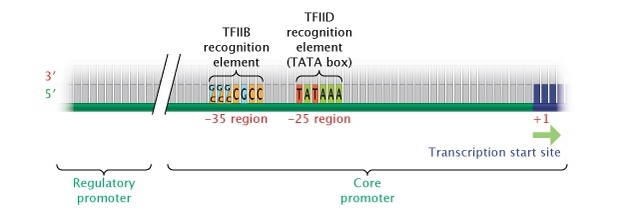
\includegraphics[width=\textwidth,natwidth=626,natheight=216]{core_promoter.jpg}
   \caption[Core promoter elements]{Core promoter elements recognised by RNA Pol II include the transcription factor IIB recognition element and the TATA box, which are located around 35 and 25 bp upstream of the transcription start site (TSS), respectively. Various regulatory elements that regulate transcription may lie further upstream. Image used with permission from Nature Education 2014.}
   \label{fig:core_promoter}
\end{figure}

Once transcription has initiated, RNA pol and its associated proteins unwind the DNA double helix; once unwound, RNA pol reads the template DNA strand and adds nucleotides to the 3' end of a nascent RNA transcript. Transcription is terminated when the RNA polymerase reaches the termination site and the mRNA transcript and RNA pol are released (Figure ~\ref{fig:transcription}). Transcription results in two main classes of RNA transcripts: (1) Protein-coding transcripts, where the RNA known as mRNA can be further translated into a protein molecule and (2) Non-coding transcripts, where the RNA molecule is the functional product and not an intermediate to proteins.

\begin{figure}[!ht]
   \centering
   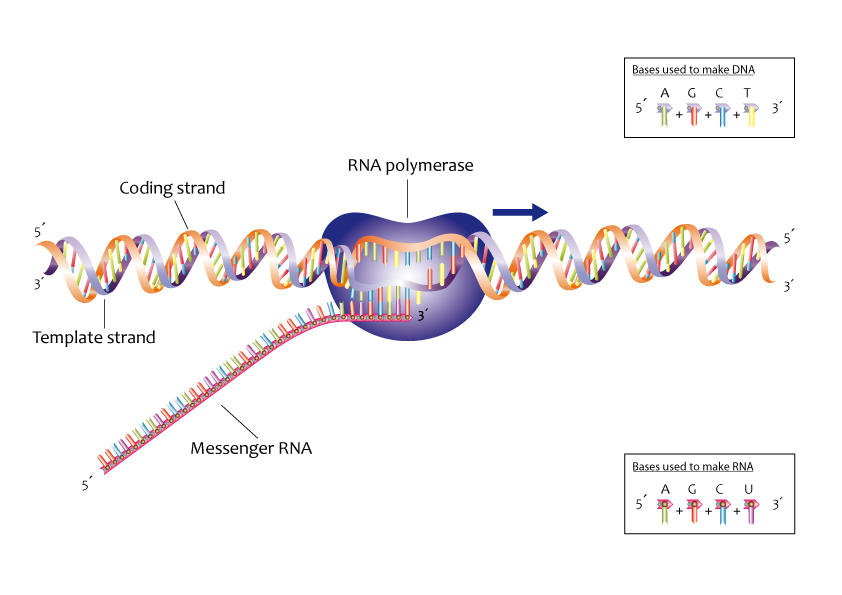
\includegraphics[width=\textwidth,natwidth=842,natheight=595,totalheight=0.70\textheight,keepaspectratio]{transcription.jpg}
   \caption[DNA transcription]{The process of transcription can be broadly grouped into three stages: a) Initiation, b) Elongation, and c) Termination. Initiation involves the binding of RNA polymerase (shown as a large green blob) to the promoter and the DNA double helix starts to separate. RNA polymerase starts reading the sequence on the template strand in the 5' to 3' direction (green arrow). The elongation step involves the movement of RNA polymerase along the DNA strand producing a growing RNA transcript chain, which continually opens and closes the DNA strand. Nucleotides are shown as pink T-shaped molecules and the red arrow indicates that they are added at the 3' end of the nascent transcript. The termination step occurs once the RNA polymerase reaches the termination site, and the RNA transcript and RNA polymerase are separated from the DNA. Image used with permission from Nature Education 2013.}
   \label{fig:transcription}
\end{figure}

\subsection{Transcriptional regulation}

In 1961, François Jacob and Jacques Monod demonstrated how genes were activated and suppressed on a molecular level, developing the theory of genetic regulation \citep{pmid13718526}. The regulation of transcription ensures that transcripts are expressed in the correct spatial and temporal manner, which is necessary for cellular diversity and for responding appropriately to environmental changes. The mechanisms governing transcriptional regulation mainly fall into two classes: those directly related to the DNA sequence and those that are not related to the DNA sequence \textit{per se}. Transcription factors (TFs), which are a class of regulatory proteins that plays a role in controlling the rate of transcription, fall into the first class. TFs characteristically contain DNA-binding domains (DBDs), which allow them to bind specifically to DNA regions, and can regulate transcription by affecting the binding of RNA polymerase, modifying histones, and by recruiting other proteins to the site that they are bound to \citep{pmid11092823}. TFs bind to either promoter or enhancer regions, which are a short region of DNA typically located thousands of nucleotides away from the promoter they interact with; this is possible as they are brought into proximity by the physical looping of DNA. In addition, enhancer sequences may be positioned in both forward and reverse orientations, and located either upstream or downstream from its associated promoter and still affect transcription. The promoter and enhancer regions are known as cis-regulatory elements (CREs) and they regulate the transcription of nearby elements, i.e. \textit{in cis}.

In contrast to regulatory mechanisms related to the DNA sequence are epigenetic regulatory mechanisms, which are any mechanism that provides a regulatory effect without altering the DNA sequence. DNA methylation is a biochemical modification, where a methyl group is covalently added to the 5' position of cytosines and it was first postulated in 1975 that DNA methylases could be used to regulate genes \citep{pmid1093816, pmid1111098}. High levels of DNA methylation typically lead to transcriptional silencing as methylated DNA physically impedes the binding of TFs and recruits proteins known as methyl-CpG-binding domain (MBDs) proteins, which further recruits additional proteins that make the DNA less accessible. In addition to biochemical modifications of DNA, epigenetic regulatory mechanisms include controlling the physical accessibility of DNA.

\subsection{DNA accessibility}

The structural compaction of DNA is a common strategy for limiting transcription, as TFs and RNA pols are unable to bind to the DNA. This compaction is mainly achieved via histones, which are a family of small and positively charged proteins that fold negatively charged DNA in the form of electrostatic interactions. The resulting DNA-histone complex is known as chromatin and possesses a fundamental repeating structure \citep{holde01111974}; this repeating unit is known as the nucleosome and forms the structural and functional unit of chromatin. Nucleosomes are structured with two of each of the following histones: H2A, H2B, H3, and H4, and forms a histone octamer that binds and wraps about 146 base pairs of DNA. The H1 histone protein binds to DNA that links nucleosomes, called linker DNA, wrapping another 20 bps of DNA and stabilising the linker DNA. Chromatin is found in two varieties: heterochromatin, which features DNA tightly wrapped into a 30 nm fibre, and euchromatin where DNA is lightly packed as nucleosomes (Figure ~\ref{fig:dna_condensed}).

\begin{figure}[!ht]
   \centering
   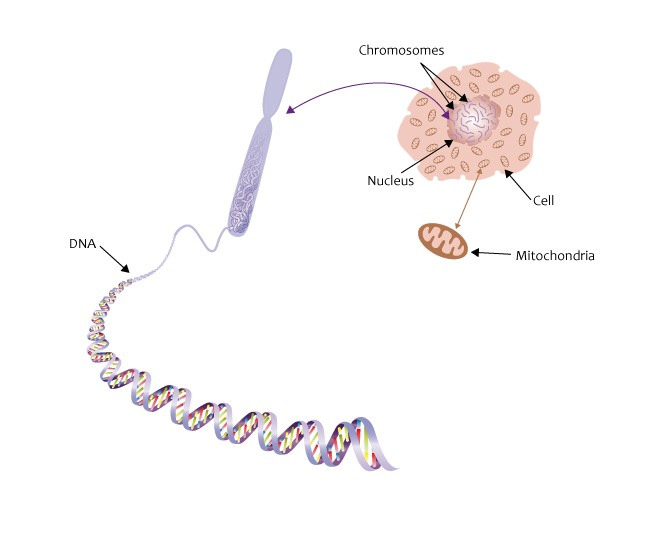
\includegraphics[width=\textwidth,natwidth=627,natheight=614]{dna_condensed.jpg}
   \caption[DNA packaging]{DNA is compacted at various levels: 1) as a double-stranded helical structure, 2 and 3) as nucleosomes, which consists of eight histone molecules with DNA wrapped around 1.65 times, 4) as a chromatosome, which consists of the nucleosome and a H1 histone, 5) as a 30 nm fiber of folded nucleosomes, 6) as looped nucleosomes that are on average 300 nm in length, 7) as compressed 300 nm fibers, producing a 250 nm fiber, and finally 8) as chromatids of a chromosome. Image used with permission from Nature Education 2013.}
   \label{fig:dna_condensed}
\end{figure}

Chromatin structure and the position of nucleosomes are altered during DNA transcription and replication to allow the machinery to access parts of the genome. Chromatin modifications are achieved by biochemically modifying the histones, which strengthen or weaken its association with DNA. Generally speaking, there are two major mechanisms by which chromatin is made more accessible via histone modifications: 1) Histones can be enzymatically modified by the addition of acetyl, methyl, or phosphate groups and 2) Histones can be displaced by chromatin remodelling complexes, thereby exposing underlying DNA sequences to polymerases and other enzymes. Importantly, these two processes are reversible and remodelled chromatin can be returned to its compact state after transcription and/or replication is complete.

Specific histone modifications are associated with different biological states; for example, acetylation removes the positive charge on histones, thereby decreasing the interaction between histones and DNA, loosening chromatin, and allowing transcriptional activation to take place. The nomenclature for histone modifications is defined by the name of the histone, followed by the single-letter amino acid abbreviation and its position, and then an abbreviation of the enzymatic modification; for example, H3K27ac indicates the acetylation of lysine 27 on H3. On the other hand, the tri-methylation of lysine 27 on histone H3, i.e. H3K27me3, is associated with the inhibition of transcription \citep{pmid21652639}. Given that distinct histone modifications can either be implicated in the activation or repression of transcription, a ``histone code" has been proposed \citep{pmid11498575} and the profiling of the histone states provides insights into the transcriptional state of a DNA region. Table \ref{table:histone_mod} summarises a list of histone modifications and variants profiled by the ENCODE project \citep{pmid22955616}.

\begin{table}[h]
   \footnotesize
   \begin{tabular}{l l p{5cm}}
%\textbf{Histone modification or variant} & \textbf{Signal characteristics} & \textbf{Putative functions}                                                                                        \\ \hline
\pbox[b]{20cm}{ \textbf{Histone modification} \\ \textbf{or variant} } & \textbf{Signal characteristics} & \textbf{Putative functions}                                                           \\ \hline
H2A.Z                           & Peak                   & Histone protein variant (H2A.Z) associated with regulatory elements with dynamic chromatin                                            \\ \hline
H3K4me1                         & Peak/region            & Mark of regulatory elements associated with enhancers and other distal elements, but also enriched downstream of transcription starts \\ \hline
H3K4me2                         & Peak                   & Mark of regulatory elements associated with promoters and enhancers                                                                   \\ \hline
H3K4me3                         & Peak                   & Mark of regulatory elements primarily associated with promoters/transcription starts                                                  \\ \hline
H3K9ac                          & Peak                   & Mark of active regulatory elements with preference for promoters                                                                      \\ \hline
H3K9me1                         & Region                 & Preference for the 5' end of genes                                                                                                    \\ \hline
H3K9me3                         & Peak/region            & Repressive mark associated with constitutive heterochromatin and repetitive elements                                                  \\ \hline
H3K27ac                         & Peak                   & Mark of active regulatory elements; may distinguish active enhancers and promoters from their inactive counterparts                   \\ \hline
H3K27me3                        & Region                 & Repressive mark established by polycomb complex activity associated with repressive domains and silent developmental genes            \\ \hline
H3K36me3                        & Region                 & Elongation mark associated with transcribed portions of genes, with preference for 3' regions after intron 1                          \\ \hline
H3K79me2                        & Region                 & Transcription-associated mark, with preference for 5' end of genes                                                                    \\ \hline
H4K20me1                        & Region                 & Preference for 5' end of genes                                                                                                       
   \end{tabular}
   \caption[Table of histone modifications]{Summary of histone modifications and variants profiled by the ENCODE project \citep{pmid22955616}.}
   \label{table:histone_mod}
\end{table}

\section{DNA sequencing}

DNA sequencing is the process of determining the exact order of nucleotides within a DNA molecule. The first generation of DNA sequencing methods (Sanger and Maxam-Gilbert sequencing) were developed in the 1970s and were very labour intensive, requiring four separate polyacrylamide gel electrophoresis (PAGE) runs, for the determining the sequence of each base. The key feature of Sanger sequencing \citep{pmid271968} was the use of chain-terminating dideoxynucleotide triphosphates (ddNTPs). The structure of a normal nucleotide (dNTP), consists of a 3' hydroxyl (OH) group in the pentose sugar; chain-terminating ddNTPs lack the OH group that is necessary for the formation of the phosphodiester bond between one nucleotide and the next during DNA strand elongation. The idea was to set up a reaction with a mixture of dNTPs [deoxyadenosine triphosphate (dATP), deoxyguanosine triphosphate (dGTP), deoxycytidine triphosphate (dCTP), deoxythymidine triphosphate (dTTP)] and a particular ddNTP in a ratio of 300:1. Most of the times, the DNA will be elongated but if a ddNTP is incorporated into the growing DNA strand, strand elongation is terminated. This results in DNA fragments of varying lengths, where the last base of these fragments is the incorporated ddNTP. By performing the same reaction using the other three ddNTPs and by loading the fragments of each reaction onto separate PAGE lanes, the DNA bases can be deduced by reading the four lanes (Figure ~\ref{fig:sanger_ladder}).

\begin{figure}[!ht]
   \centering
   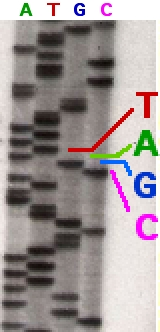
\includegraphics[width=\textwidth,natwidth=160,natheight=332,totalheight=0.20\textheight,keepaspectratio]{sanger_ladder.jpg}
   \caption[Radioactively labelled sequencing gel]{PAGE, which has a 1 bp resolution, is used to separate the radioactively labelled DNA fragments from each reaction using specific chain-terminating ddNTPs. By reading the DNA fragments, the sequence of the DNA can be deduced. Image used under the terms and agreement of the Wikipedia GFDL.}
   \label{fig:sanger_ladder}
\end{figure}

The Maxam-Gilbert sequencing method \citep{pmid265521} relies on the use of chemicals that can cleave specific bases in contrast to chain-terminating ddNTPs. Dimethyl sulfate was used to cleave purine bases (A and G) and hydrazine was used to cleave pyrimidine bases (C and T). To distinguish the purines, an adenine-enhanced cleavage step is carried out, which cleaves adenines preferentially. To distinguish the pyrimidines, NaCl is used with hydrazine to suppress the reaction of thymines. As with Sanger sequencing, the DNA fragments are separated using PAGE, and the DNA bases are deduced by reading the gel.

Sanger sequencing became the \textit{de facto} method for DNA sequencing due to its comparative ease and its use of fewer toxic materials than Maxam-Gilbert sequencing. A further improvement to Sanger sequencing replaced the need to radioactively label the DNA fragments by using chemically synthesised fluorescent oligonucleotide primers \citep{pmid3713851}. Four different fluorophores were used for each ddNTP reaction allowing all four reactions to be co-electrophoresed and the DNA sequence was deduced by reading the fluorescence colours (Figure ~\ref{fig:sanger_sequencing}). The development of a fluorescence detection apparatus linked to a computer that processed the data created the world's first partially automated DNA sequencer \citep{pmid3713851}; this development was key towards the success of the Human Genome Project (HGP). For over 25 years since its inception, Sanger sequencing has been the method of choice for DNA sequencing.

\begin{figure}[!ht]
   \centering
   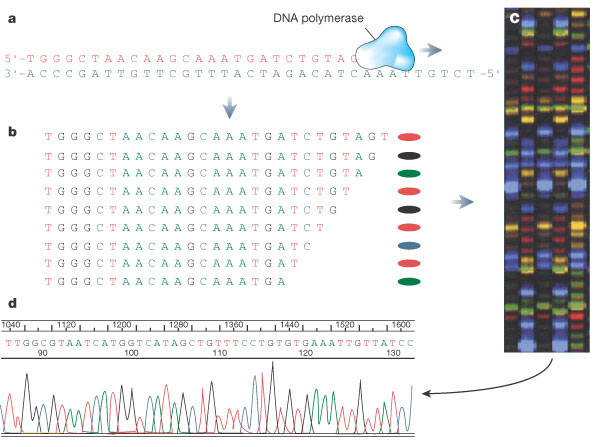
\includegraphics[width=\textwidth,natwidth=600,natheight=447]{sanger_sequencing.jpg}
   \caption[Sanger sequencing]{a) DNA polymerase synthesises a complementary strand of DNA, however when a b) fluorescently labelled chain-terminating ddNTP base is incorporated, synthesis terminates producing DNA fragments of various sizes. c) As each terminator are fluorescently labelled with different dyes, each fragment will fluoresce a particular colour and the d) sequence trace is read by a computer that determines the sequence based on the coloured peaks.}
   \label{fig:sanger_sequencing}
\end{figure}

\subsection{Next-generation sequencing}

The next wave of DNA sequencing techniques, the so-called next-generation (next-gen) or second generation sequencing, started with various strategies that relied on a combination of template preparation, sequencing, and imaging that allowed thousands to billions of sequencing reactions to be performed simultaneo-usly \citep{pmid19997069}. Next-gen sequencing relies on the clonal amplification of templates and uses \textit{in vitro} cloning rather than bacterial cloning; the two most common methods of clonal amplification are emulsion polymerase chain reaction (emPCR) \citep{pmid12857956} and solid-phase amplification \citep{pmid16473845}. With emPCR individual DNA molecules are isolated with primer-coated beads in water-in-oil microreactors and clonal amplification leads to thousands of copies of the DNA molecule in an emulsion. 454 pyrosequencing and Sequencing by Oligonucleotide Ligation and Detection (SOLiD) sequencing employ emPCR and the amplification products are deposited into individual wells for sequencing. Solid-phase amplification relies on a lawn of high-density primers that are covalently attached on a slide surface (also known as a flow cell) and bind to DNA molecules that have been ligated with sequencing adaptors. The two methods allow each DNA template to be spatially separated and allow massively parallel sequencing to take place.

Sequencing can take place via the use of DNA polymerase, which is commonly known as sequencing-by-synthesis (SBS), or via the use of DNA ligase, which is known as sequencing-by-ligation (SBL). SBS can be further classified into cyclic reversible termination (CRT), single-nucleotide addition (SNA), and real-time sequencing \citep{pmid19997069}. CRT uses reversible terminators and initial developments used the dideoxynucleotides chain terminators implemented in Sanger sequencing. The concept of CRT is that a DNA polymerase incorporates one fluorescently modified nucleotide, which has a reversible terminator that terminates DNA synthesis. Unincorporated nucleotides are washed away and fluorescence imaging takes place to determine the identity of the incorporated nucleotide. The last step removes or cleaves the reversible terminator and the fluorescent dye, and the cycle is repeated. The CRT method is used in Solexa/Illumina and Helicos single-molecule fluorescent sequencing. SBL relies on DNA ligase and uses either one-base-encoded or two-base-encoded probes that are fluorescently labelled. The probes hybridise to its complementary sequence on the primed template and DNA ligase is added to join the probe to the primer. Non-ligated probes are washed away followed by fluorescence imaging and cleavage of the fluorescent dye and the cycle is repeated. The SBL method is used in SOLiD sequencing.

\subsection{Third generation sequencing and beyond}

The third generation of sequencing refers to single-molecule sequencing technologies, which has the capacity for generating longer read lengths at potentially cheaper costs \citep{pmid20858600}. One of the major advantages of single-molecule sequencing is that polymerase chain reaction (PCR) is not required, and therefore amplification biases and PCR mutations are eliminated. Furthermore, by employing third generation sequencing, quantitative applications of sequencing, such as RNA sequencing, can give a much more representative picture of the true abundance of RNA molecules. The HeliScope sequencer was the first commercially available single-molecule sequencer, which was based on the work of Stephen Quake and colleagues \citep{pmid12651960}. HeliScope sequencing utilises billions of primed single-molecule templates that are covalently attached to a solid support and uses CRT but with slight differences from Solexa/Illumina sequencing. HeliScope sequencing uses Helicos Virtual Terminators, which differ from the reversible terminators used in Solexa/Illumina sequencing and dye labelled nucleotides are added individually in the predetermined order of C, T, A, and G, followed by fluorescence imaging.

With the advent of high-throughput sequencing we now have the capacity to sequence an entire human genome in a matter of days. In addition, we have just recently arrived in the \$1,000 genome era, whereby we can sequence the entire genome of an individual at a 30x depth (the minimum depth required for clinical applications) for around 1,000 US dollars (USD). In contrast, the HGP, which gave us the first glimpse of the human genome \citep{lander2001initial} costed approximately 2.7 billion fiscal year 1991 US dollars \citep{nhgri2010cost}. Further developments in sequencing by various companies are aiming towards longer read lengths at a higher output (Figure ~\ref{fig:dev_next_gen}). Currently, different sequencers either have very long reads but at a low-throughput or have a high-throughput of shorter reads; as such, each sequencer fills a particular niche. \textit{De novo} assembly of genomes requires longer reads for less ambiguity and the quantification of RNA requires higher throughput in order to accurately sample the vast RNA population.

\begin{figure}[!ht]
   \centering
   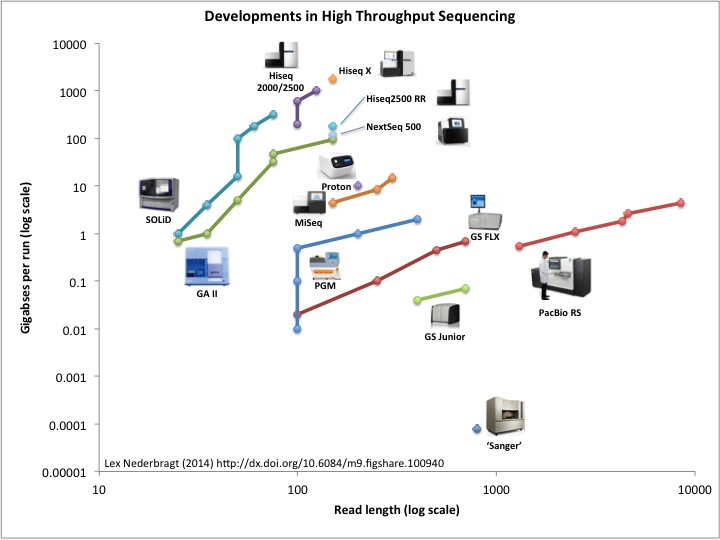
\includegraphics[width=\textwidth,natwidth=720,natheight=540]{developments-in-next-generation-sequencing.jpg}
   \caption[Developments in next generation sequencing]{Read length ($ log_{10} $) versus gigabases per run ($ log_{10} $) for various high-throughput sequencer \citep{Nederbragt2012}. Currently, the HiSeq X, the sequencer that bought us into the \$1,000 genome era, provides the highest throughput. Image used under the terms and agreement of the CC-BY license.}
   \label{fig:dev_next_gen}
\end{figure}

\section{Expression analysis}

The binding and positioning of RNA pol to a region of DNA results in transcription and the subsequent ``expression" of an RNA transcript. A transcript may be constitutively expressed, i.e constantly expressed, or expressed according to the current cellular requirements. By comparing the expression levels of transcripts between different conditions, hypotheses can be generated on the possible function/s of a particular transcript. Northern blotting \citep{pmid414220} was one of the first methods for quantifying the expression level of specific RNA transcripts. This technique involves the electrophoretic separation of purified RNA, followed by immobilising the RNA onto a blotting membrane; detection of the transcript is achieved by hybridising a specific probe that is complementary to part of the transcript. The relative amount of a specific transcript can be estimated by comparing the strength of signals from different samples; this estimate assumes that an equivalent amount of total RNA was used per sample and this is verified by using a probe that detects a constitutively expressed transcript. Northern blotting is also useful for determining the size of a specific transcript and is commonly used for detecting alternatively spliced transcripts; however, Northern blotting is not very sensitive for estimating transcript abundance.

The most sensitive method of detecting specific transcript levels is quantitative real-time polymerase chain reaction (qRT-PCR), which is able to detect sparse levels of transcripts, down to the level present in single cell. The method employs the use of a fluorescent dye and PCR, where the primer pairs are designed to be specific for a given transcript. By measuring the number of cycles that is required for the formation of a detectable amount of product, which is known as the cycle threshold ($C_{t}$) value, the transcript levels can be estimated by comparing the results to qRT-PCR experiments performed using standard samples \citep{pmid11846609}; lower $C_{t}$ values indicate higher amounts of initial template. It should be ensured that the PCR step is equally efficient for different transcripts by proper primer design, as a more efficient PCR will result in a lower $C_{t}$ value compared to a less efficient PCR.

Methods that measure transcript levels inside a cell use this quantification as a proxy for the expression level. However, it should be pointed out that various factors affect transcript levels, such as post-transcriptional modifications. Transcript stability is one primary factor, as transcripts that are rapidly degraded may appear to be lowly expressed. Specific biological experiments need to be implemented in order to differentiate between an unstable transcript or a lowly transcribed transcript, for example by knocking down proteins involved in RNA degradation \citep{pmid19056938}. Another point to consider is the stochastic nature of transcription \citep{pmid17048983}, whereby transcripts are produced in bursts.

\subsection{Transcriptome profiling}

Transcriptome profiling refers to the expression profiling of the complete collection of transcripts in a cell at a specific time point. Transcripts associated with a particular biological process or disease state can be identified by profiling all transcripts and in addition, the interplay between transcripts can be inferred by studying transcripts with similar expression patterns. One of the first technologies that allowed the simultaneous profiling of thousands of transcripts at once were microarrays \citep{pmid7569999}. DNA probes that are complementary to specific DNA sequences, such as complementary DNAs (cDNA) or genomic regions, are attached to a solid surface and fluorescently labelled target sequences are hybridised onto the surface. Target sequences that complement the probe sequences hybridise to the probe and the signal intensity provides a measure of the expression strength of a particular transcript. In one of the first application of microarrays, researchers were able to observe the change in expression levels of 700 mRNAs during a switch from aerobic to anaerobic respiration in yeast cells \citep{pmid9381177}. However, microarrays have several limitations, which includes requiring \textit{a priori} knowledge of the genome or transcript sequences, high background levels from cross-hybridisation \citep{pmid16749918}, and a limited dynamic range in quantifying expression.

In contrast to the hybridisation approach of microarrays, sequencing-based approaches have been developed for transcriptome profiling. Prior to the advent of next-gen sequencing, sequencing approaches were based on the sequencing of short tags; these tagging approaches were cost-effective, as only short fragments of cDNAs were sequenced. Typically type IIS restriction enzymes were used to create tags, which were then concatenated, cloned, and sequenced. A technology called Serial Analysis of Gene Expression (SAGE) \citep{pmid7570003} was the first tag-based approach, which created 13 to 14 bp long tags (including the restriction site of the anchoring enzyme). These tags corresponded to the most 3' portion of a cDNA where a restriction site for the anchoring enzyme would be present. A similar technology known as Massive Parallel Signature Sequencing (MPSS), was later developed, which is similar to SAGE but employs different biochemical steps and a different sequencing approach \citep{pmid10835600}. MPSS was an improvement to SAGE in that it produced longer tags (16-20 bp) and libraries that were 20 times larger than typical SAGE libraries \citep{pmid10835600}. Another tagging method known as the paired-end ditag (PET) approach, prepared ditags that corresponded to the 5' and 3' end of the same full-length cDNA \citep{pmid15782207}. The PET approach allows the mapping of cDNA boundaries, helps resolve ambiguous tag mappings by using the paired-end information, and has the potential to detect unconventional fusion transcripts and rearrangement events. The SAGE approach also gave rise to Cap Analysis Gene Expression (CAGE) \citep{pmid14663149}, which combines the tagging strategies of SAGE with a molecular technique known as Cap-Trapper \citep{pmid8938445,pmid9179497}. The CAGE protocol captures all capped transcripts and sequences a short tag (20 or 27 nt depending on which restriction enzyme is used) that corresponds to the 5' end of an RNA transcript (Figure ~\ref{fig:cage_protocol}).

\begin{figure}[!ht]
   \centering
   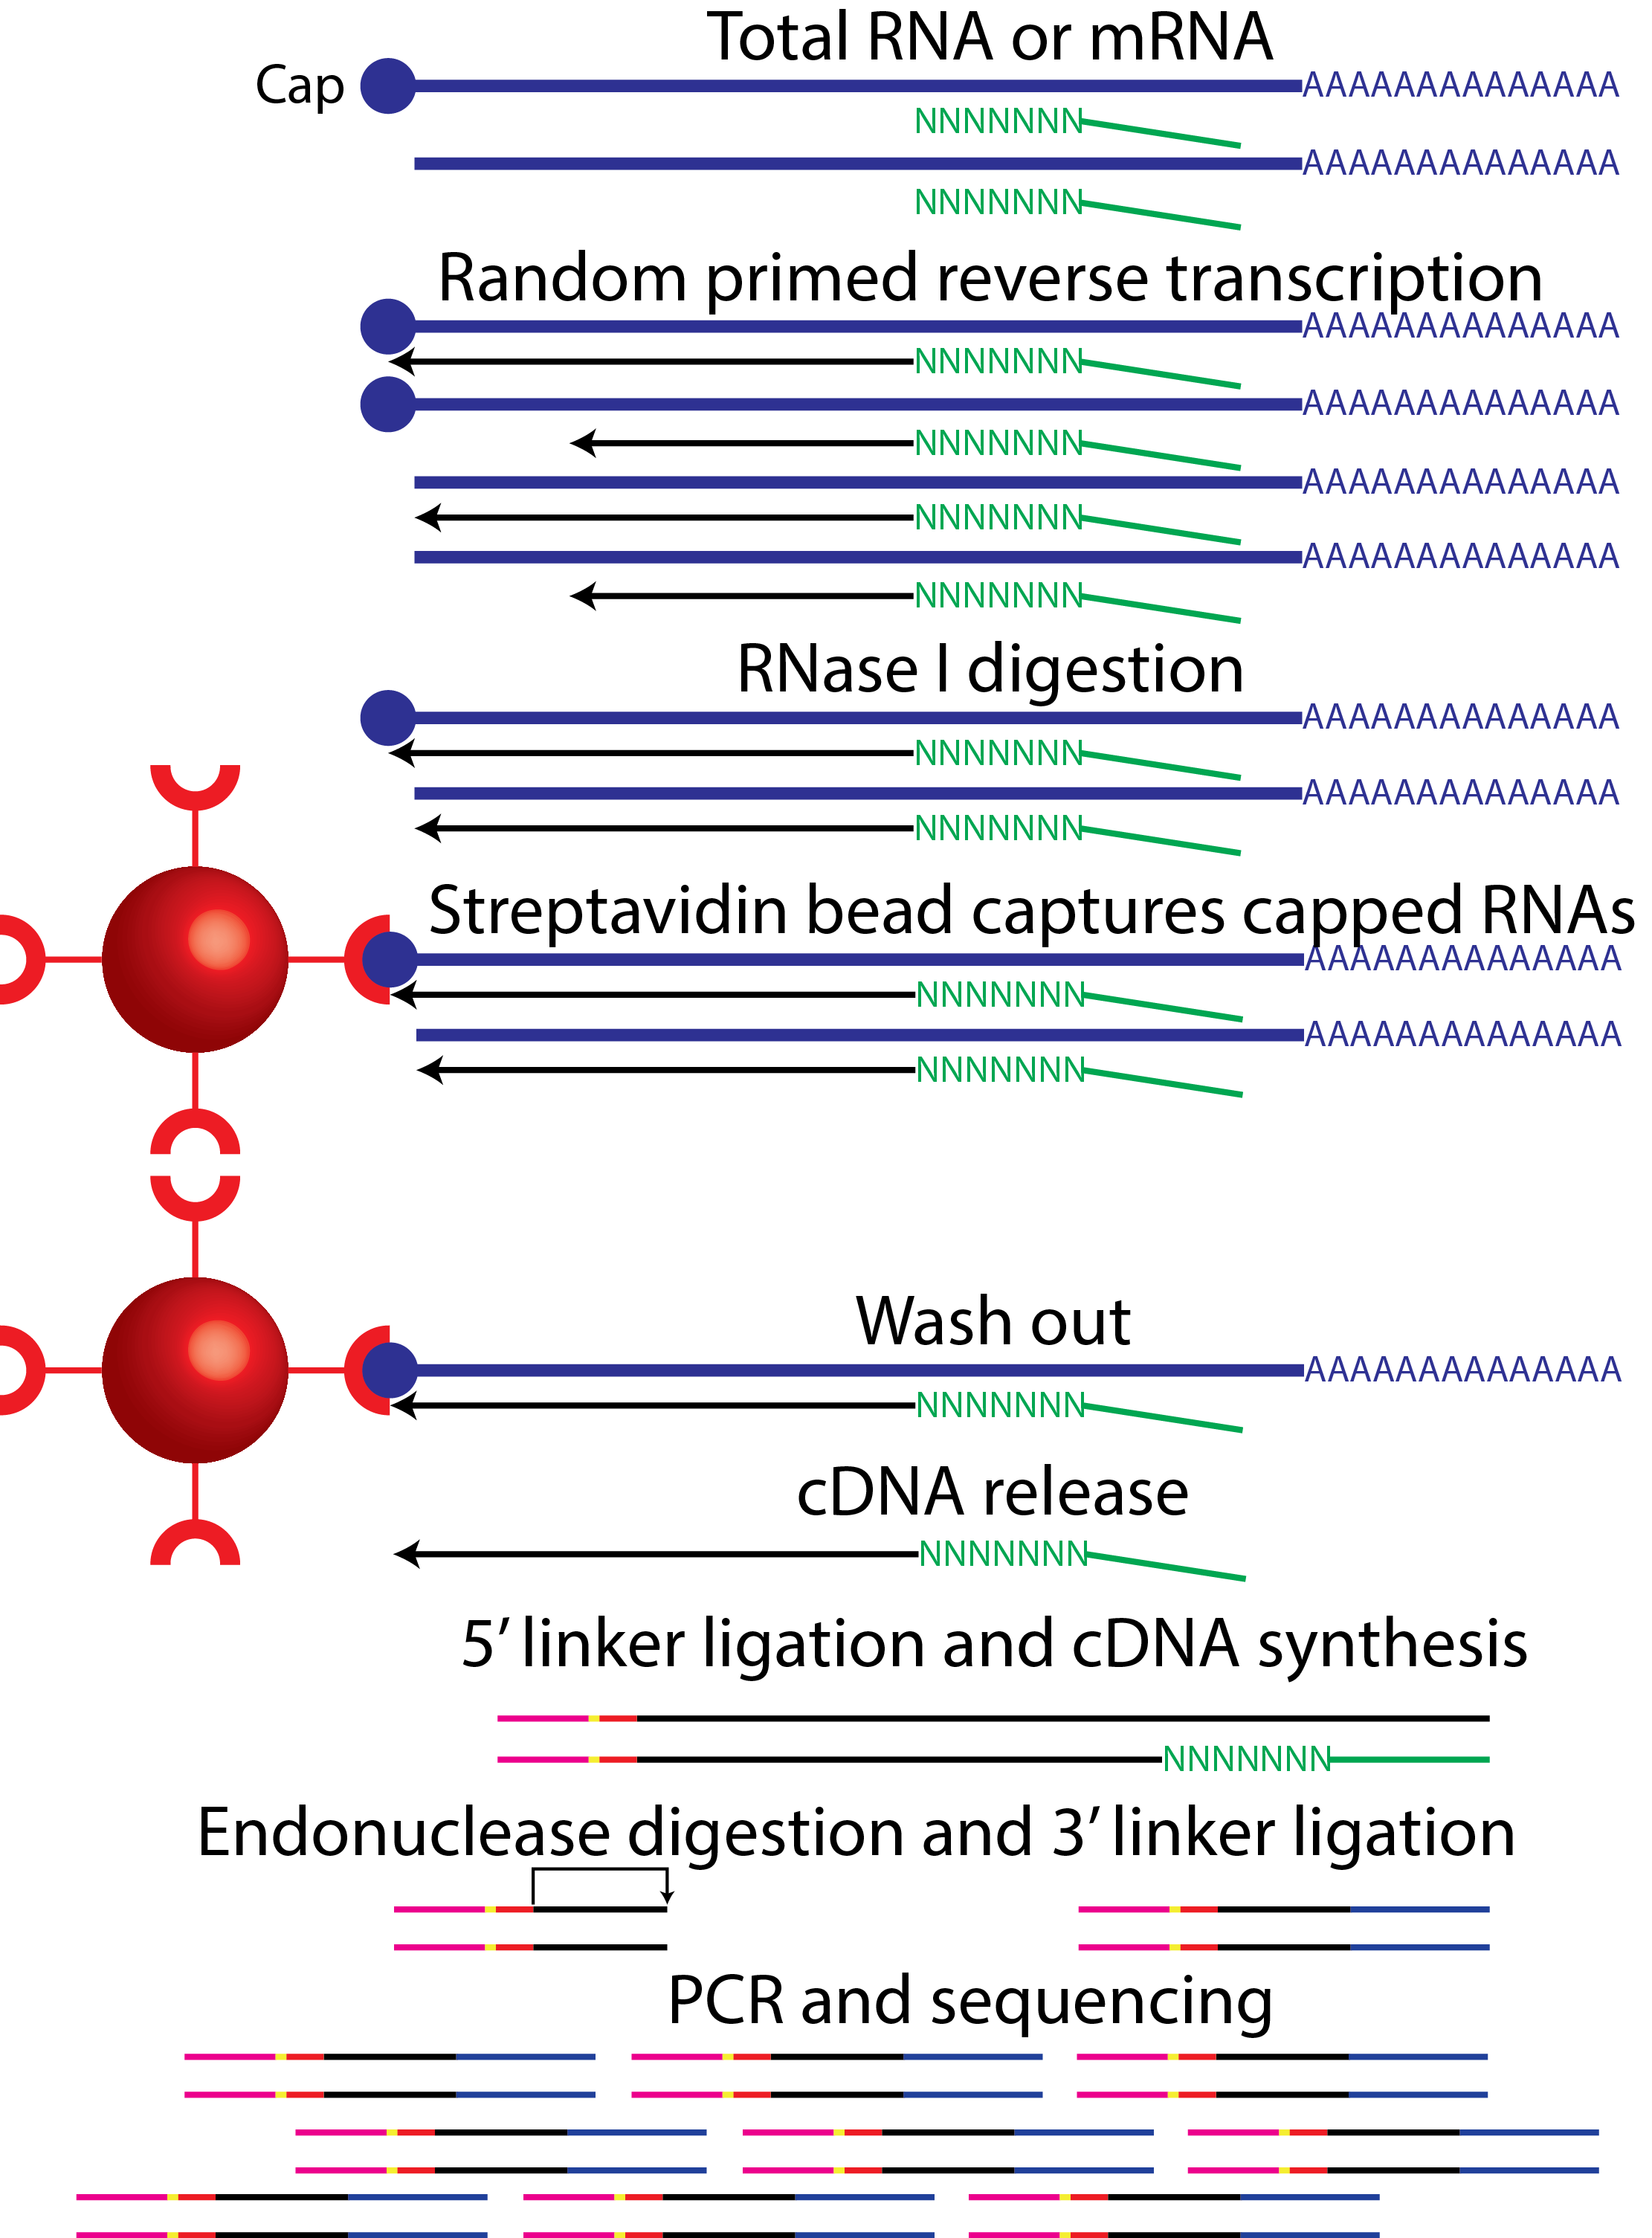
\includegraphics[width=\textwidth,natwidth=2254,natheight=3051,totalheight=0.65\textheight,keepaspectratio]{cage_protocol.png}
   \caption[Cap Analysis Gene Expression protocol]{The tagging Cap Analysis Gene Expression (CAGE) protocol starts with synthesising cDNA from either total RNA or mRNA by using random or oligo dT primers (only random primers are shown here). Reverse transcription takes place in RNAs with or without a cap and to full or partial completion; the RNase I digestion step removes partially reverse transcribed RNA as they are not protected by a full double strand. The 5' end of cDNAs are selected by streptavidin beads that capture the biotin labelled cap structure and unbound cDNA are washed out. After release from the bead, a linker is attached to the 5' end of the single-stranded cDNA; this linker contains a barcode sequence (in yellow) followed by a recognition site (in red) that allow the endonuclease digestion. Lastly a linker is ligated to the 3' end of the tag sequence (in blue), which is amplified and directly sequenced.}
   \label{fig:cage_protocol}
\end{figure}

With the arrival of next-gen sequencing, the SAGE and CAGE methods were adapted to high-throughput sequencers \citep{pmid14676315,Takahashi2012}. The short-read and high-throughput nature of next-gen sequencing suited tag-based approaches aptly, as the tag lengths were in the size range of reads produced by the sequencer. Whole transcriptome shotgun sequencing or simply RNA sequencing (RNA-Seq) methods were later developed to sequence entire populations of RNA. RNA-Seq refers to the fragmentation of RNA followed by deep-sequencing on next-gen sequencing platforms \citep{pmid19015660}; the fragmentation step is required due to the short-read nature of next-gen sequencers. Typically, RNA-Seq methods enrich for transcripts with a poly-A tail; this enrichment step is carried out to avoid rRNA sequences, which make up a large fraction of the total RNA population. One major difference between RNA-Seq and the tag-based approaches is that the entire length of the RNA is sequenced in RNA-Seq; the advantage in this is that alternative splicing patterns can be inferred. However tag-based approaches, such as CAGE, can be used in a complementary nature to RNA-Seq \citep{pmid24676093}, since transcript boundaries are defined clearly in CAGE.

\subsection{Transcriptional complexity}

Several landmark studies have revealed that the transcriptional landscape is much more complex than previously anticipated. The functional annotation of the mammalian genome (FANTOM) project, which began as an initiative to sequence and functionally annotate mouse full-length complementary DNA (cDNA) \citep{pmid11217851}, revealed that the transcriptome was dominated by transcripts that had no apparent coding potential \citep{pmid12466851}. The FANTOM consortium also revealed massive antisense transcription \citep{pmid16141073}, which is transcription arising from the strand opposite the sense strand, and extensive alternative promoter usage \citep{pmid16141072}. Tiling arrays, which are microarrays designed to interrogate a genome at evenly spaced intervals, revealed that a large fraction of genomic bases were transcribed \citep{pmid15539566, pmid11988577, pmid15790807}. This observation that a large percentage of mammalian genomes are transcribed became known as pervasive transcription \citep{pmid17510325}, however these claims made on the basis of tiling arrays were questioned \citep{pmid20502517}. However, the Encyclopaedia of DNA elements (ENCODE) project, which endeavours to identify all functional elements in the human genome, observed that mammalian genomes were pervasively transcribed \citep{pmid17571346, pmid22955616}. These claims were based on the use of various genome-wide biochemical assays and multiple lines of evidence. However, it is not known whether these products of transcription are functional or not, as they do not overlap known genes.

\subsection{Defining a gene}

The idea of a gene dates back to Gregor Mendel and his plant breeding experiments that demonstrated that discrete traits could be inherited from parents to offspring. The term ``gene" was coined in 1909 by Wilhelm Johannsen to describe the Mendelian units of heredity. Genes were later described as the precursors to proteins, in the ``one gene, one polypeptide" hypothesis, when it was observed that mutations in Neurospora genes would cause defects in different steps of metabolic pathways  \citep{Beadle15111941}. After the determination of the genetic code (see section~\ref{sec:central_dogma}), a gene was recognised as a stretch of DNA that coded for a protein in an open reading frame (ORF). The discovery of introns \citep{pmid890740,pmid922889}, altered the ORF concept, in that genes were now composed of both protein-coding regions (exons) and the non-coding regions (introns). The trend had been that each time a major discovery had been made, the definition of a gene was revised. Thus in light of pervasive transcription members of the ENCODE consortium suggested that the definition of a gene needs to be updated yet again \citep{pmid17567988}. The definition they proposed was: ``A gene is a union of genomic sequences encoding a coherent set of potentially overlapping functional products" \citep{pmid17567988}. This definition is similar to the idea of a transcriptional unit (TU), proposed by the FANTOM consortium, which is a segment of the genome that shares common core of genetic information and is able to generate transcripts \citep{pmid12466851}.

\subsection{Non-coding RNAs}

The protein-centric view of genes segregated RNA as either being coding RNA, the mRNAs, or RNA with no coding potential, known as ncRNAs. Historically, it was believed that there were only a few ncRNA families, such as the tRNAs, rRNAs, and the spliceosomal RNAs, all of which aided the processing of proteins. NcRNAs exist as single-strand nucleic acid molecules, which tend to fold on themselves due to the hydrophobic nature of bases, to form localised double-stranded regions that form structures called hairpins or stem-loop structures. NcRNAs can be broadly classified as short or small RNAs, which are defined as being \textless200 nucleotides long, or as long non-coding RNAs (lncRNAs), which are \textgreater200 nucleotides in length; these size cut-offs correspond to the commonly used size selections in biochemical fractionations and does not have any biological implications.

One of the most well studied classes are the micro-RNAs (miRNAs), which were first observed in \textit{Caenorhabditis elegans} \citep{pmid8252621}. MiRNAs are typically 20-24 nucleotides in length and function as regulators of expression by base-pairing with complementary sequences within mRNAs (commonly to the 3' untranslated region (UTR)). The biogenesis of miRNAs begins with the transcription of the miRNA gene by either RNA pol II or pol III, forming the primary miRNA (pri-miRNA). The pri-miRNA is then cleaved by an enzyme called Drosha \citep{pmid14508493} to produce a characteristic stem-loop structure of about 70 bps, known as the precursor miRNA (pre-miRNA). The pre-miRNA is then exported into the cytoplasm and is further cleaved by an enzyme called Dicer \citep{pmid11201747}, producing the functional mature miRNA. Another class of well known ncRNAs are the piwi-interacting RNA (piRNA), which were first observed in drosophila \citep{pmid11470406}. PiRNA are typically between 24 and 32 nucleotides long and are mainly involved in silencing transposable elements (TEs) by guiding the piwi-type proteins to complementary sequences on the TEs \citep{pmid18282709}. The biogenesis of piRNA is currently unclear, however, a ping-pong cycle has been proposed, where a primary processing pathway generates the primary piRNAs, and an amplification cycle amplifies the primary piRNAs \citep{pmid21427766}.

The lncRNAs are not as well characterised as miRNAs or piRNAs and are defined as transcribed RNAs with no coding potential and described with respect to protein-coding genes (sense, antisense, bidirectional, intronic, and intergenic) \citep{pmid19239885}. LncRNAs have been dismissed due to lack of sequence conservation \citep{pmid15495343} and have been suggested to be products of transcriptional noise \citep{pmid15851066}. However, several lines of evidence including conserved secondary structure, context-specific transcription patterns, and splicing patterns suggest that a subset of lncRNAs are may be functional \citep{pmid19188922}. However, while there has been several well documented cases of lncRNAs, it has been suggested that more experimental work needs to be done to reveal how many lncRNAs are indeed functional \citep{pmid23463798}.

The list of ncRNAs (Table \ref{table:ncRNAs}) has increased over the last 20 years due to technological advances, such as RNA-Seq. These include, but are not limited to, promoter upstream transcripts \citep{pmid19056938}, long intergenic non-coding RNAs \citep{pmid21890647, pmid22196729, pmid2943744}, transcription start site-associated RNA \citep{pmid21822281}, enhancer RNAs \citep{pmid20393465}, promoter-associated short RNAs and termini-associated short RNAs \citep{pmid17510325}, double strand break-induced small RNAs \citep{pmid22445173} or DNA damage RNAs \citep{francia2012site}, competing endogenous RNAs \citep{pmid24429633}, and transcription initiation RNAs \citep{pmid19377478}. Despite an abundance of ncRNA classes, many of these ncRNAs are supported only by transcriptional data, since validation studies have only been performed in a low-throughput manner. As the genome is pervasively transcribed, transcription by itself is not enough evidence to support function. Newer technologies, such as parallel analysis of RNA structure \citep{pmid20811459} and fragmentation sequencing \citep{pmid21057495}, that focus on the structural properties of RNA may provide more clues to the extent of functionality of ncRNAs.

\begin{table}[h]
   \footnotesize
   \begin{tabular}{p{3cm} l p{5cm}}
\textbf{Non-coding RNA}                       & \textbf{Typical size (bp)} & \textbf{Putative functions}              \\ \hline
Transcription initiation RNA                  & 17-18                      & Transcriptional regulation               \\ \hline
Micro-RNA                                     & 20-24                      & Silencing of targeted messenger RNA      \\ \hline
DNA damage RNA                                & 22-23                      & Establishing the DNA damage response     \\ \hline
Promoter-associated short RNA                 & 22-200                     & Unknown                                  \\ \hline
Piwi-interacting RNA                          & 24-32                      & Silencing of transposable element        \\ \hline
Enhancer RNA                                  & 50-2000                    & Transcriptional regulation               \\ \hline
Transfer RNA                                  & 73-94                      & Translation of messenger RNA             \\ \hline
Long intergenic non-coding RNA                & \textgreater200            & Chromatin modification                   \\ \hline
Ribosomal RNA                                 & 1,900 and 5,000            & Protein synthesis                        \\ \hline
Competing endogenous RNA                      & Undefined                  & Micro-RNA sponge                         \\ \hline
   \end{tabular}
   \caption[Table of non-coding RNAs]{A list of various non-coding RNAs, their size profiles, and putative functions.}
   \label{table:ncRNAs}
\end{table}

\section{Repetitive mammalian genomes}

The discovery that cells contained a large fraction of repetitive DNA was made by measuring the re-association rates of DNA strands after denaturation \citep{Britten1968}. The characterisation of repetitive elements (REs) was possible with the release of the mouse \citep{pmid12466850} and human \citep{venter2001sequence, lander2001initial} genome sequences, which showed that these genomes are indeed largely made up of REs. The two major groups of REs are tandem repeats, which include different classes of satellite repeats, and interspersed repeats, which are mostly made up of transposable elements (TEs) \citep{pmid9666329}. Within TEs are two main classes: Class I TEs or retrotransposons, which are DNA elements that are transcribed into RNA, reverse transcribed back to DNA, and transposed to a new location in the genome (a copy-and-paste mechanism), and Class II TEs or DNA transposons, which simply excise their DNA sequence from one location to another via transposase enzymes (a cut-and-paste mechanism). As retrotransposons are able to produce a copy of themselves before propagation, they are more numerous than DNA transposons. The retrotransposon known as the Alu element, has an estimated copy number of more than one million, making them the most abundant RE in the human genome \citep{lander2001initial}.

There are various methods for identifying REs in genomes, which can be broadly categorised into \textit{de novo}, homology, structure, and comparative genomic based methods \citep{Bergman01112007}. For the initial mouse and human genome sequencing projects, REs were catalogued using a popular software called RepeatMasker, which identifies REs by using homology-based methods to search against a database of consensus repeats \citep{pmid19274634}, such as the Repbase Update database \citep{pmid16093699}. One of the main drawbacks of identifying REs in this manner is the reliance on sequence homology and a single consensus sequence, resulting in missing REs with an extensive number of mutations. Recently, RepeatMasker has incorporated the use of profile Hidden Markov Models to annotate REs \citep{pmid23203985}; profile methods use an alignment of multiple representative sequences rather than a single consensus and are more sensitive than single sequence searches. However, REs not contained within databases may still be missed and \textit{de novo} methods may be the key to identifying these repeats. It has been proposed that up to two-thirds of the human genome may be made up of repetitive elements based on a \textit{de novo} identification method \citep{pmid22144907}.

\subsection{Junk DNA}

Historically, TEs have been labelled as purely selfish elements that have no function or provide no selective advantage to an organism \citep{doolittle1980selfish, orgel1980selfish} and were considered as junk DNA. The term ``junk DNA", was popularised by Susumu Ohno \citep{pmid5065367}, who used it to describe pseudogenes, which are gene copies that have no known biological function. In its modern day usage, ``junk DNA" is used to describe DNA sequence that does not play a functional role in an organism. The question of how much of the human genome is functional was also addressed by Susumu Ohno, who used a fixed mutation rate (each locus has a $10^{-5}$ probability of sustaining a deleterious mutation) to estimate the number of functional loci \citep{pmid5065367}. Given this mutation rate, he predicted that the human genome could not have more than 30,000 loci under selection, as this would guarantee a progressive decline in genetic fitness, leading to mutational meltdown \citep{pmid24809441}. In stark contrast to the estimation made by Susumu Ohno, the ENCODE project reported that 80\% of the human genome has a biochemical function \citep{pmid22955616}, to which junk DNA was immediately dismissed \citep{Pennisi07092012}. This lead to several critiques \citep{pmid23431001, pmid23479647, Eddy2012}, which all raised the issue of whether biochemical activity is enough to assert function.

One peculiar observation among eukaryotic genome sizes, known as the C-value enigma, is the lack of correlation between genome sizes and organismal complexity \citep{pmid11325054}. The genome size variation among eukaryotes can be partially explained by the presence or absence of TEs \citep{pmid12188048}, which raises the question of whether or not these sequences are necessary or simply junk. To answer this question, the \textit{Fugu rubripes} genome was sequenced to provide a useful reference for annotating functional elements in the human genome \citep{pmid12142439}. The fugu has one of the smallest vertebrate genomes; at 390 Mb less than 10\% of the genome is made up of REs, compared to 50\% in the human genome (Figure ~\ref{fig:repeat_coverage_vertebrate_genome}). An even more extreme example, is the genome of the carnivorous bladderwort plant, \textit{Utricularia gibba}, which is 82 Mb in size and is almost devoid of REs \citep{pmid23665961}. At least in these two organisms, their genomes suggest that ``junk DNA" is not essential.

\begin{figure}[!ht]
   \centering
   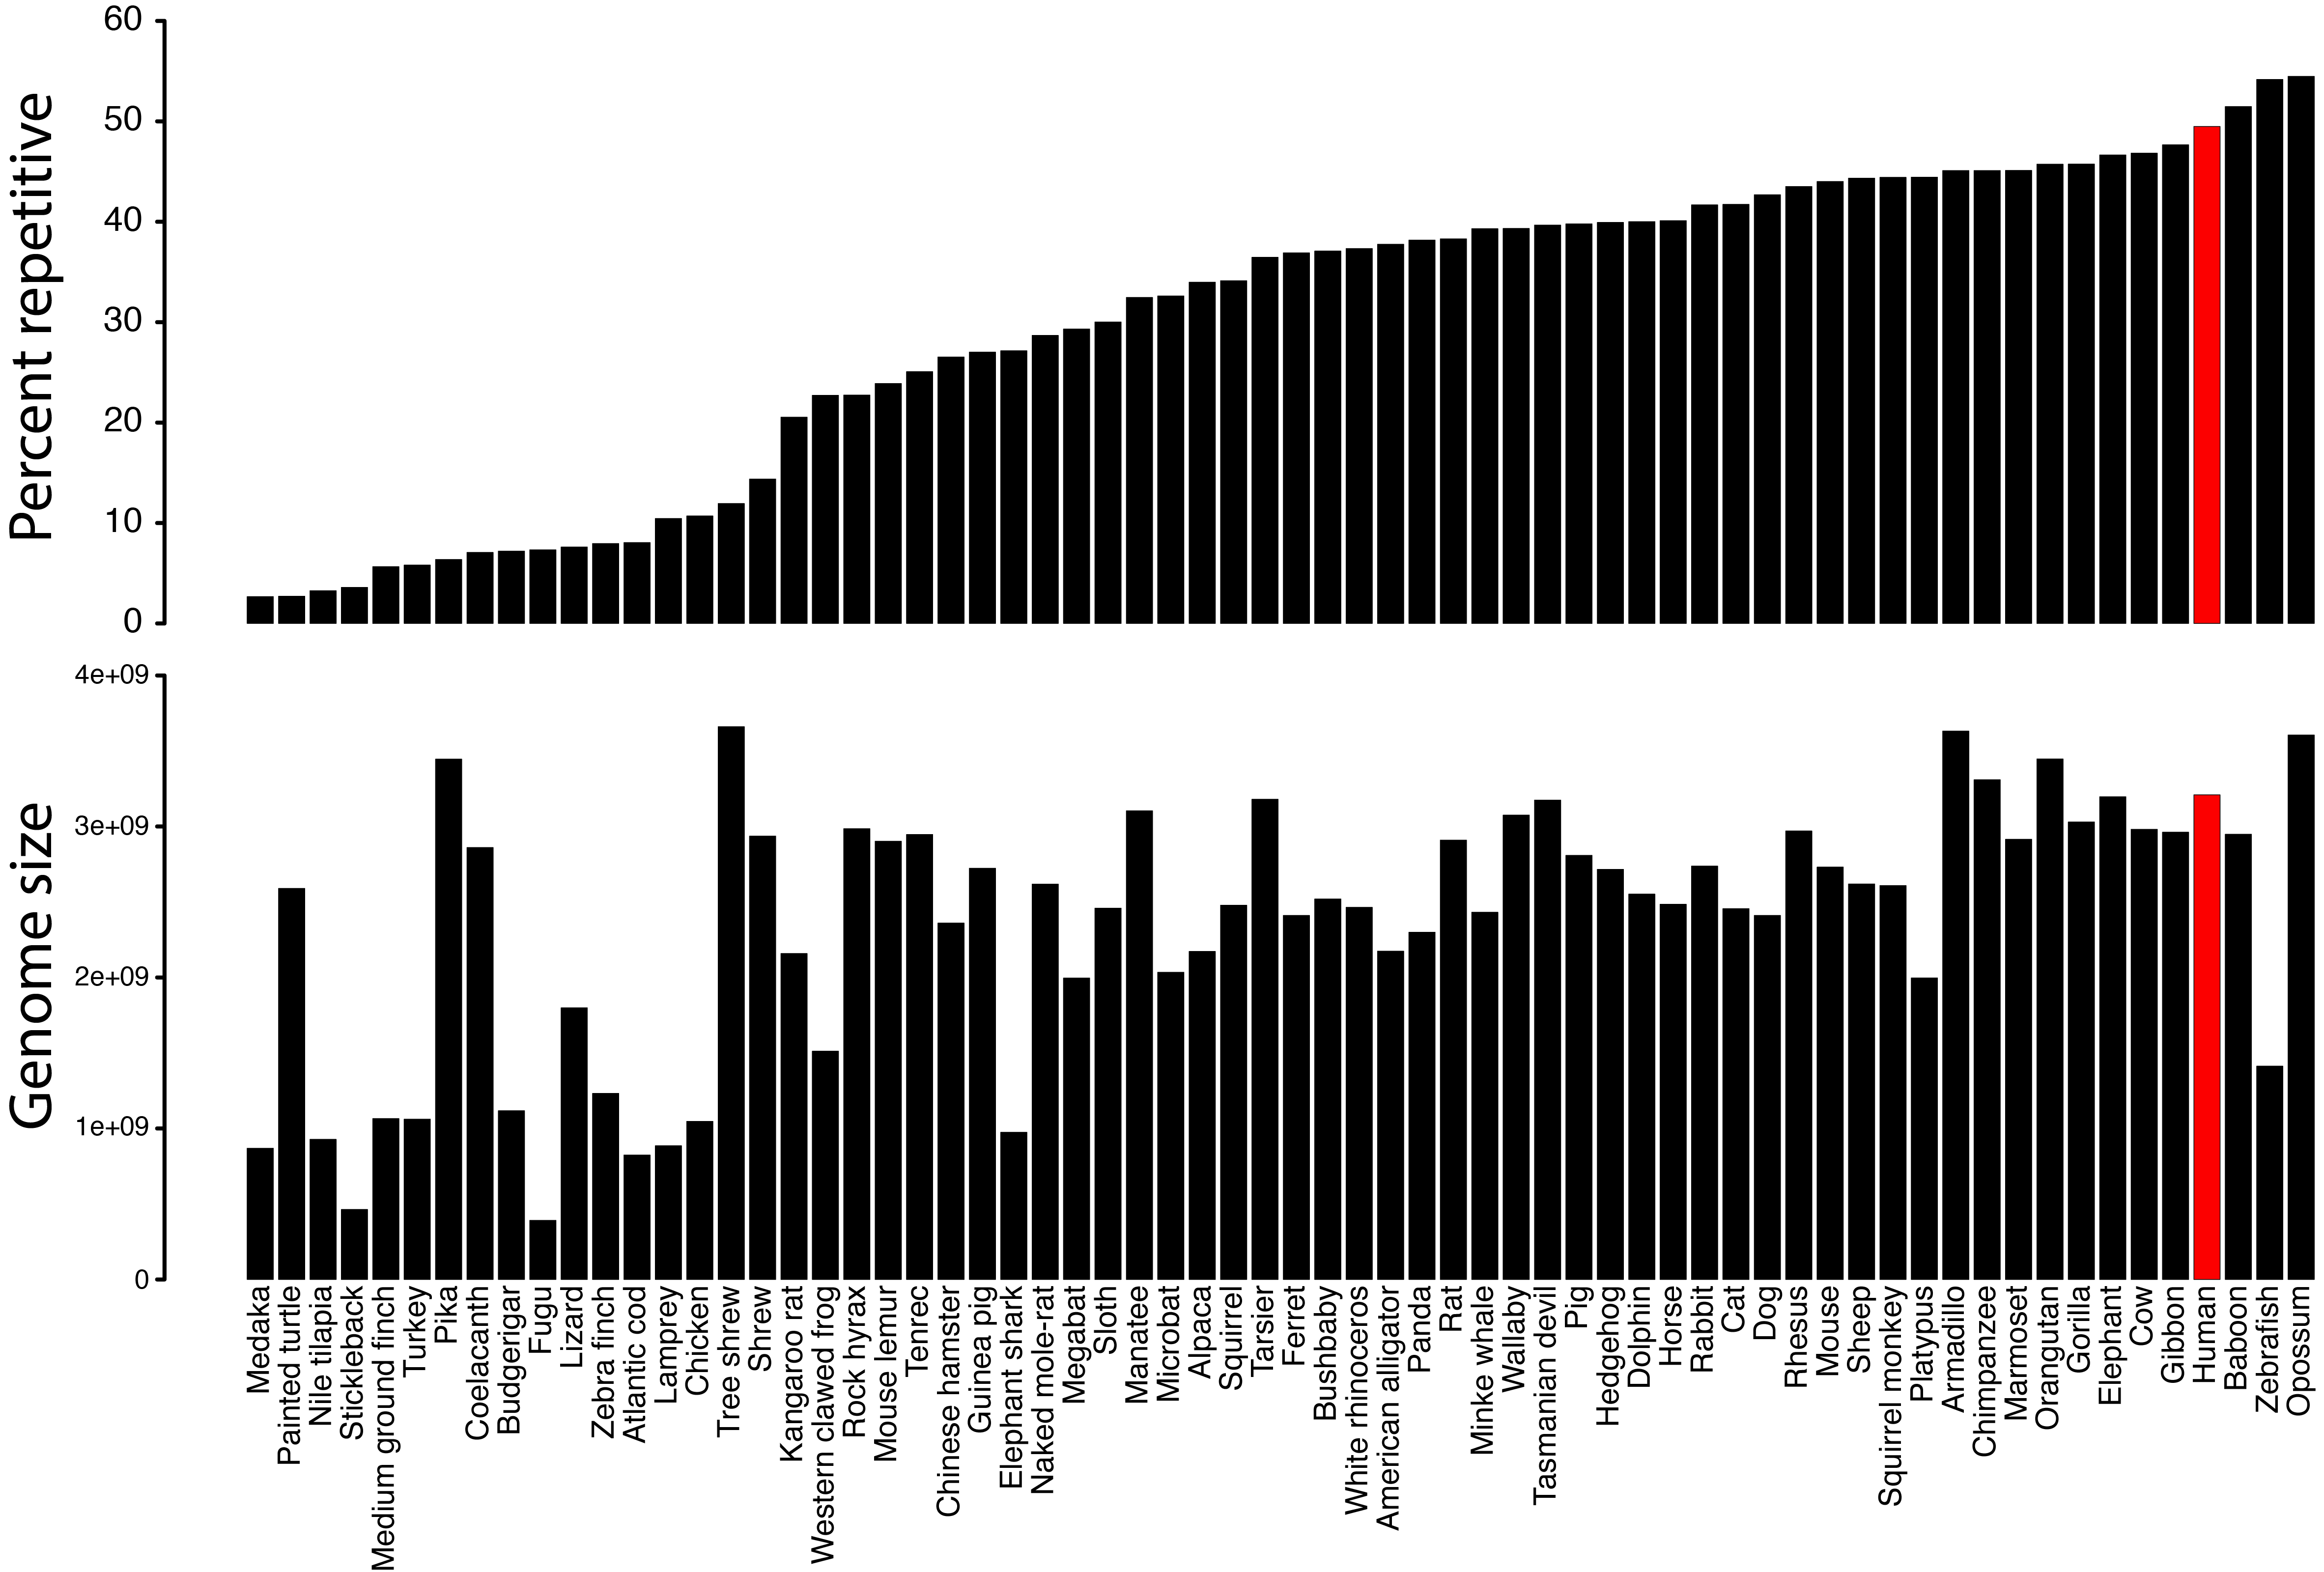
\includegraphics[width=\textwidth,natwidth=4730,natheight=3200]{percent_and_genome_size.png}
   \caption[Coverage of repetitive elements in vertebrate genomes]{The total coverage, in percentage, of repetitive elements in 66 vertebrate genomes as annotated by RepeatMasker and their respective genome sizes in base pairs; the human genome is shown in red \citep{tang2014repcoverage}. Image used under the terms and agreement of the CC-BY license.}
   \label{fig:repeat_coverage_vertebrate_genome}
\end{figure}

\subsection{Impact of transposable elements on genomes}

Genome evolution has been largely affected by TEs, which have the ability to move around within genomes. The activity of TEs have led to insertion mutations and genomic instability, but have also contributed to genetic innovation \citep{pmid19763152}. Despite the dismissal that TEs are purely selfish and are non-essential elements, the possibility that some TEs may become useful was speculated:

\epigraph{``It would be surprising if the host genome did not occasionally find some use for particular selfish DNA sequences, especially if there were many different sequences widely distributed over the chromosomes. One obvious use $\ldots$ would be for control purposes at one level or another. This seems more than plausible."}{--- \textup{Orgel and Crick 1980}}

While the estimated number of active TEs in the human genome is less than 0.05\% \citep{pmid17331616}, it is clear that TEs have impacted the evolution of genomes. There is increasing evidence that TEs have served as a source for evolutionary innovation by contributing to the evolution of regulatory networks \citep{pmid18368054}, influenced alternative splicing \citep{pmid18818740}, drove the evolution of lncRNAs \citep{pmid23637635}, and provided alternative promoters for genes \citep{pmid19577618}. These examples illustrate the process of exaptation, where a character (the TE) becomes co-opted for a new function that it was not originally functional for \citep{Gould01011982}. As speculated by Orgel and Crick, there may be many other examples of TE exaptation, however, large-scale analysis of TE expression have been limited. This was due to cross-hybridisation problems with repetitive sequences in microarrays and the short read nature of current high-throughput sequencers.

In one of the first genome-wide profiling studies of TE expression, it was revealed that a large number of transcriptional events initiate within TEs in a tissue specific manner \citep{pmid19377475}. Many of these TSSs were validated experimentally to show that TEs served as alternative promoters. In order to deal with the multi-mapping nature of reads corresponding to TEs, a probabilistic method called multi-map rescue was implemented \citep{pmid18178374}, which allowed reads to be assigned probabilistically based on the nearby region. Another genome-wide study examining the methylation patterns of TEs revealed tissue-specific methylation patterns \citep{pmid23708189}. In this study, the authors developed the Repeat Analysis Pipeline (RAP), to deal with ambiguously mapped reads, in a manner that aggregates reads to families of repeats \citep{pmid20584328}. Both of these studies illustrate the importance of developing specific methodologies for analysing TEs and that TEs have been important in regulating the expression of genes.

\section{Bioinformatics and genomics}

Modern day high-throughput sequencers generate a large amount of data and dedicated informatics tools for storing, managing, and the analysis of such data sets are absolutely necessary. Bioinformatics can be thought of as a subset of informatics that deals with biological data, though historically it was defined as ``the study of informatic processes in biotic systems" \citep{pmid21483479}. The HGP was one of the first large scale international research efforts, which demonstrated how bioinformatics was crucial towards the successful completion of the project \citep{stein1996perl}. Furthermore, the HGP also set the stage for data sharing by establishing important principles, known collectively as the ``Bermuda Principles", that promoted the rapid and public sharing of human genome information. These set of commitments left a lasting legacy in large genomic science projects such as The International HapMap Project, ENCODE and modENCODE, and The Cancer Genome Atlas, where data are made freely available prior to publication \citep{contreras2011bermuda}. By opening such resources, researchers are able to integrate and leverage these datasets for generating testable hypothesises.

While many of the foundations in bioinformatics were related to molecular evolution and population genetics, the availability of complete genome sequences has opened up an entire research discipline called genomics. The field of genomics is also closely tied with bioinformatics, as genomics studies typically deals with large amounts of data, corresponding to features of genomes. There are several sub-branches within genomics; the field of functional genomics focuses on the dynamic aspects of genomes, such as transcription, interactions between proteins and genomic regions, and DNA methylation patterns. Functional genomics, as the name suggests, attempts to discover and establish function to elements in the genome and usually employing the use of high-throughput methods for genome-wide screening.

\subsection{High-throughput sequencing data}

The FASTQ format was formally defined in 2010 \citep{pmid20015970} and has become the \textit{de facto} format for storing raw high-throughput sequencing data. FASTQ is similar to the FASTA format but with the addition of quality scores, known as the Phred quality score, for each sequenced nucleotide and is usually the starting point of bioinformatic pipelines. Typically, quality control (QC) steps are carried out next to remove potential artefacts and low quality reads; one such tool known as TagDust \citep{pmid19737799}, removes reads that match sequences used during the library preparation, such as primer and adaptor sequences. Other QC steps include removing reads containing undetermined bases, as they indicate poor overall read quality; for sequencers that output reads of different lengths, reads outside the main length distribution are removed; quantifying highly over-represented 10-mers can also be implemented as a QC step \citep{pmid21088025}, to identify potential artefactual sequences.

In order to put sequencing reads into context, reads are mapped onto their corresponding reference genome; various tools are available for aligning high-throughput sequencing reads. Traditional tools such as BLAST \citep{pmid2231712} and BLAT \citep{pmid11932250} are unable to cope with the large quantity and short length of reads from high-throughput sequencers. One popular short-read alignment tool, BWA \citep{pmid19451168}, implements the Burrows–Wheeler transform to deal with millions to billions of short reads. The Burrows-Wheeler transform allows a large mammalian genome, for example human, to be indexed and stored efficiently into memory \citep{pmid19430453}. The Sequence Alignment/Map (SAM) format \citep{pmid19505943} is the standard file format for storing sequence alignments and contains all the information for reconstructing an alignment. In addition the SAM format contains information on where a read maps on the genome, the quality of the mapping, and depending on the alignment program, other mapping statistics. The open source program SAMTools \citep{Li15082009}, provides various utilities for the processing and analysis of alignments stored in the SAM format. In order to save disk space, SAM files are typically stored as BAM files, which are simply their binary equivalent. Recent developments have introduced a newer format known as CRAM, based on a newer compression method \citep{pmid21245279}, which further compresses BAM files but are still processable using SAMTools.

The BED format is another standard file format used for storing the location of a set of features (or even sequencing reads) with respect to a reference genome and has been popularised by the UCSC Genome Browser \citep{Kent01062002}. Due to the popularity of the BED format, a suite of tools released as BEDTools \citep{pmid20110278}, provides various routines for comparing genomic features stored in BED format. A common task in processing RNA-Seq data involves intersecting mapped reads to known genomic features, such as genes, to associate a read to a gene and thereby quantifying its expression. In addition to this, the proximity of elements on a chromosome may indicate potential functional interactions, thus reads may be annotated with respect to the physical distance, i.e. spatially, to genomic features. For example, promoters are usually upstream and nearby the genes that it initiates transcription for, thus CAGE reads are associated with nearby gene models in this manner.

\subsection{Analysing expression datasets}

Expression data sets are typically represented as matrices; for example, if we let $A$ be an $m \times n$ matrix, where $a_{ij}$ are elements of $A$, then the $i^{th}$ row would represent the transcriptional response of the $i^{th}$ transcript and the $j^{th}$ column would represent the expression profile of the $j^{th}$ assay:

\begin{align*}
   A = \begin{bmatrix} a_{11} & \cdots & a_{1j} & \cdots & a_{1n} \\
   . && . && . \\
   a_{i1} & \cdots & a_{ij} & \cdots & a_{in} \\
   . && . && . \\
   a_{m1} & \cdots & a_{mj} & \cdots & a_{mn} \end{bmatrix}
\end{align*}

Typically, two or more groups of assays are produced, such as a set of control experiments versus a set of treated experiments, and the aim is to find differentially expressed transcripts between the two conditions. Data normalisation is required prior to comparing assays to ensure that experimental factors (not including the experimental treatment) that cause differences are accounted for. For example, a library that has been sequenced twice as much as another library will have most of its transcript as seemingly expressed twice as much. One way to account for this is to normalise reads by counts or tags per million (TPM); to normalise by TPM the $i^{th}$ gene in the $j^{th}$ assay:

\begin{align*}
   TPM_{a_{ij}} = \frac{a_{ij} \times 1000000}{\sum_{i=1}^{m}{a_{mj}}}
\end{align*}

Other methods include normalising the expression by the length of a transcript, known as reads per kilobase of transcript per million mapped reads or fragments per kilobase of transcript per million mapped reads, for RNA-Seq experiments where reads are generated throughout the length of the transcript, quantile normalization, which is a technique for making two distributions identical in statistical properties \citep{pmid12538238}, and trimmed mean of M values (TMM), which is a normalisation method that takes into account differences in the RNA population from different samples by scaling the expression \citep{pmid20196867}.

After the appropriate normalisation methods have been carried out, the testing of differential expression is performed by comparing the amount of variation between groups against the amount of variation within groups for a particular transcript, which is similar to carrying out a \textit{t}-test or analysis of variance (ANOVA). However, the simple assumptions of these tests are not met due to the heteroscedastic and non-normal distribution properties of high-throughput sequencing data. RNA-Seq expression is measured by digital counts of reads, meaning that expression levels are discrete, and the variance is modelled using discrete probability distributions. In a pioneering study examining the reproducibility of RNA-Seq, it was noted that the variation between technical replicates was close to the shot noise limit \citep{pmid18550803}. Thus it was suggested that the Poisson model was sufficient in modelling the variance and used for testing differential expression. However, it was demonstrated that the Poisson model underestimated the effects of biological variability, i.e. the variation between two different biological samples is greater than Poisson variation \citep{20979621}. This can be accounted for by modelling variance under a negative binomial model, which has been implemented for differential expression analysis in the edgeR package \citep{pmid19910308} from Bioconductor \citep{pmid15461798}.

The correlation of transcriptional responses or expression profiles can be calculated to identify transcripts expressed in a similar manner or assays with a similar profile, respectively. Correlation measures such as Pearson's product-moment correlation coefficient or Spearman's rank correlation coefficient are typically used and can be used as a measure of co-expression, i.e. transcripts with a similar transcriptional response are assumed to be co-expressed. Other measures of similarity or rather dissimilarity include metrics such as the Euclidean, maximum, Manhattan, Canberra, Jaccard, and Minkowski distances. Hierarchical clustering is usually performed in an agglomerative manner to reveal the topology of distance matrices and visualised using dendrograms to revealing the most similar transcripts or assays. The visualisation of expression datasets include heatmaps, which transforms the expression matrix into colours representing the relative expression strength and are commonly arranged according to the hierarchical clustering structure \citep{pmid9843981}. Graphs can also be used to represent associations of transcripts or assays, which can leverage methodologies developed in graph theory.

Expression datasets are usually large and therefore subjected to the multiple testing problem, whereby significant p-values are observed due to the large number of statistical inferences that are carried out. Several techniques are used to account for this, such as the Bonferroni correction or false discovery rate (FDR) control \citep{fdr_paper} and these techniques generally require a higher p-value significance threshold to compensate for the number of inferences made. A FDR of 10\% means that it is expected that 10\% of our statistical inferences are false positives and the FDR is the p-value at which to draw a threshold. It is important to account for multiple testing when performing numerous statistical tests, which is common when analysing high-throughput expression datasets.

\section{Research goals}



Early studies employing the use of tiling arrays suggested that mammalian genomes are largely transcribed, which became known as pervasive transcription \citep{pmid17510325}. However, the findings from tiling arrays were criticised on the basis that the technology was noisy, i.e. probes may be able to hybridise without perfect complementary, and thus over-estimated the extent of transcription \citep{pmid20502517}. High-throughput transcriptome sequencing, which is also known as RNA-Seq, sequences the total RNA population of a sample and provides a much more comprehensive profile of the transcriptome. A comprehensive survey of transcriptomes using RNA-Seq on various cell lines indeed confirmed that the genome is pervasively transcribed \citep{pmid22955620}. The interpretation of pervasive transcription has been a topical topic in the field and has been controversial.

In this thesis, we analyse the data output from various high-throughput transcriptome sequencing results.

In this thesis, we will employ the use of high-throughput sequencing to study the transcriptional output of various biological systems with the specific aim of relating the output to the respective systems.

This approach is a discovery-driven one (in contrast to a hypothesis-driven one), where transcriptome data will be generated and analysed for differential expression.

The basic assumption of these studies is that differences under a specific set of conditions will be manifested in the transcriptome and can be captured by various high-throughput sequencing protocols.

The comparison of various transcriptomes will allow the identification of specific transcripts that are differentially expressed in distinct cell or tissue types, or in different conditions, and in turn will allow us to generate hypotheses on the role of specific transcripts in various biological systems.



